\subsection{The Kruskal extension \textbf{N}}
		\begin{figure}[htbp]
			\begin{center}
				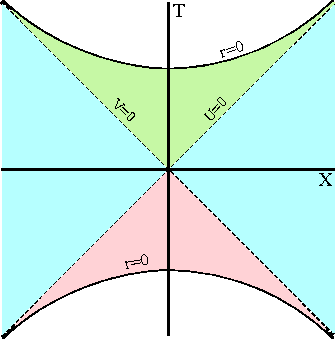
\includegraphics[scale=1]{kruskal}
			\end{center}
			\caption{This is the $XT$ plane of the \textbf{Kruskal extension}. The horizons are the dashed lines. The blue wedges are the exterior, the green wedge is the future interior and the past interior is in red. Nothing can escape the green wedge into the blue wedges, because there is no radial null geodesic which would connect the wedges.}\label{kruskal}	
		\end{figure}
	From here on, we will use $r_{s}=2GM=1$.
	Instead of using the coordinates $(t,r,\Omega)$ like in the previous section, we now introduce the Kruskal-Szekeres coordinates, because they are a better choice for near-horizon physics.
	
	First we parametrize the radial null geodesics in the Schwarzschild geometry as
		\begin{equation}
			t=\pm r_{*} + C,
		\end{equation}
	where C is some constant of motion and $r_{*}$ is a new radial coordinate defined as
		\begin{equation} \label{r_*tortoise}
			r_{*}\equiv r+\log (r-1).
		\end{equation}
	also called the \textit{tortoise coordinate}\footnote{The name \textit{"tortoise"} has its origin in the paradoxon of with Achilles and the tortoise.}, because now we have an infinite coordinate range that fits in a finite geodesic distance.
		
		Now, the Kruskal-Szekeres coordinates are defined as
		\begin{equation}
			U\equiv -e^{\frac{r_*-t}{2}}
		\end{equation}
		\begin{equation}
			V\equiv e^{\frac{r_*+t}{2}}.
		\end{equation}
	%\clearpage			%vllt mal Marei fragen, wie man das besser mit den footnotes machen kann
	Their lines of constant U and V are radial null geodesics and these coordinates have the feature, that
		\begin{equation}
			 UV=(1-r)e^r.
		\end{equation}
	This means we have a singularity at $UV=1$ and the horizon is at $U=0$ or $V=0$. The metric looks now like
		\begin{equation}
			\diff s^2=-\frac{2}{r}e^{-r}\left(\diff U \diff V + \diff V \diff U\right)+r^2 \diff \Omega^2_{2}
		\end{equation}
	Because this metric still has an off-diagonal tensor, we define another set of coordinates
		\begin{equation}
		\begin{split}
			U=T-X 	\\	
			V=T+X
		\end{split}
		\end{equation}
	Now the metric looks as follows:
		\begin{equation}\label{SchXT}
			\diff s^2=\frac{4}{r}e^{-r}\left(- \diff T^2+ \diff X^2\right)+r^2 \diff \Omega^2_2
		\end{equation}
	Note that there is now no singularity at $r=1$.
	
	This metric defines a geometry over the full XT plane, which looks like Figure \ref{kruskal}. The right blue wedge is, in the old Schwarzschild coordinates, former $r>1,~-\infty<t<\infty$ HIER FEHLT NOCHWAS. \marginpar{left blue wedge too?}
		
		For $r<1$ we are in the green region for $T>0,~X^2-T^2<0$ and in the red wedge for $T<0$ and still $X^2-T^2<0$. 
